\chapter{Functional programming and computational effects at scale}
~\label{cpt-effects}

This chapter presents and discusses ``Student's Big Brother'' --- a distributed
system to support study workflow in a programming class. It was designed to help
teachers to distribute their attention to all students uniformly. The system consists
of client daemons, watching students activity and sending their source code to a server
in real"/time (over HTTP), for storage, processing and displaying in teacher web"/interface.
The source code is freely available on GitHub~\cite{sbbRepo}.

The system is mostly implemented using Haskell programming language and the implementation
extensively uses monad transformers and extensible effects --- the concepts discussed previously
in this thesis --- to structure the necessary side"/effects and separate the effectful
functionality from the pure code.

The rest of the chapter is structured as follows: the first section gives a short
note on motivation for the system's creation; the second section abstractly describes
the system's architecture; the third section focuses on implementation details:
configuration files, integration and deployment and benefits of the use of functional
programming; the last section reports the system usage in real"/life teaching.

\section{Motivation}

It is unfortunate, but most undergraduate students hesitate to ask questions during
programming practice sessions. Usually, the instructing teacher is fighting
students' shyness by walking around the room, observing students and trying to
determine whether the particular student is succeeding or not. But due to the
limited time of the sessions and the fact that there is only one instructor per
10"/15 students, the described procedure is quite inefficient. Besides, teacher's
status checks may interrupt the string students who don't need the support. To approach the
problem, we propose to build a real"/time monitoring system of students activities during
programming classes. This system should have features of basic
version control and of displaying the students' source code in a lightweight
web"/interface for the instructor to be able to observe the activity of every
student in real"/time.

The primary purpose of the system is to distribute teachers attention between
all the active students uniformly and to help the teacher to determine which one
needs an assistance but hesitates to ask for it.

\section{System's architecture}

\usetikzlibrary{shapes, arrows, calc, positioning}

\tikzset{
    module/.style={
           rectangle,
           rounded corners,
           draw=black, very thick,
           minimum height=2em,
           inner sep=2pt,
           text centered,
           },
}


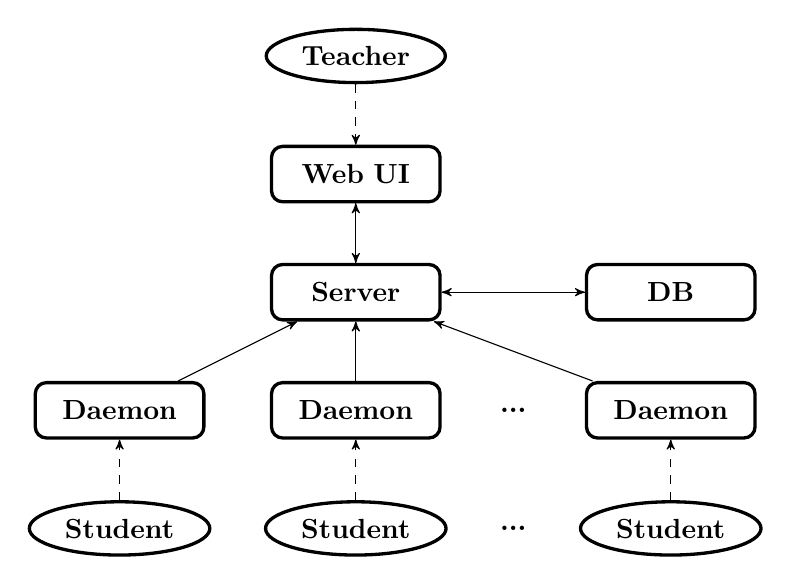
\begin{tikzpicture}[->,>=stealth']

 \node[ellipse, draw=black, very thick] (TEACHER)
 {%
  \textbf{Teacher}
 };

 \node[module,
  yshift=-0.5cm,
  text width=2cm,
  below of=TEACHER] (UI)
 {%
  \textbf{Web UI}
 };

 \node[module,
  text width=2cm,
  yshift=-0.5cm,
  below of=UI] (SERVER)
 {%
  \textbf{Server}\\
 };

 \node[module,
  below of=SERVER,
  yshift=-0.5cm,
  xshift=-3cm,
  anchor=center,
  text width=2cm] (DAEMON_1)
 {%
  \textbf{Daemon}
 };

 \node[module,
  right of=DAEMON_1,
  xshift=2cm,
  text width=2cm] (DAEMON_2)
 {%
  \textbf{Daemon}
 };

 \node[module,
  right of=DAEMON_2,
  xshift=1cm,
  draw=none,
  text width=1cm] (HIDDEN_DAEMONS)
 {%
  \textbf{...}
 };

  \node[module,
  right of=HIDDEN_DAEMONS,
  xshift=1cm,
  text width=2cm] (DAEMON_3)
 {%
  \textbf{Daemon}
 };

 \node[module,
  right of=SERVER,
  xshift=3cm,
  text width=2cm] (DB)
 {%
  \textbf{DB}
 };

 \node[ellipse, draw=black, very thick,
       below of=DAEMON_1,
       yshift=-0.5cm, ] (STUDENT_1)
 {%
  \textbf{Student}
 };

  \node[ellipse, draw=black, very thick,
       below of=DAEMON_2,
       yshift=-0.5cm, ] (STUDENT_2)
 {%
  \textbf{Student}
 };

  \node[ellipse,
       below of=HIDDEN_DAEMONS,
       yshift=-0.5cm, ] (HIDDNE_STUDENT)
 {%
  \textbf{...}
 };

  \node[ellipse, draw=black, very thick,
       below of=DAEMON_3,
       yshift=-0.5cm, ] (STUDENT_3)
 {%
  \textbf{Student}
 };

 \path (DAEMON_1) edge (SERVER);
 \path (DAEMON_2) edge (SERVER);
 \path (DAEMON_3) edge (SERVER);

 \path (SERVER) edge (DB);
 \path (DB) edge (SERVER);

 \path (SERVER) edge (UI);
 \path (UI) edge (SERVER);

 \path (TEACHER) edge[dashed] (UI);

 \path (STUDENT_1) edge[dashed] (DAEMON_1);
 \path (STUDENT_2) edge[dashed] (DAEMON_2);
 \path (STUDENT_3) edge[dashed] (DAEMON_3);

\end{tikzpicture}

The system consists of three software components: the server, the client daemon and the
teacher's web user interface (UI). The communication between all participants is performed
over HTTP using JSON"/formatted messages.

The rest of this section gives a more detailed account of the role of every component.

\subsection{Daemon: data collector}

The client daemon is a data collection agent. It is designed to run silently on
a student's computer, observe student's activity and report it to a server.

The daemon's operation protocol is simple: it runs on a student's computer,
watches the working directory for changes in source code files and regularly sends
these changes to the application server for storage and distribution.

\subsection{Server: data keeper and distributor}

The server's role is to be the central authority for the daemons: collect the files
the send, store them in a database and give them to the web UI on demand.

The server's code is essentially a CRUD"/service~\cite{Martin:1983:MDB:538746} ---
it implements creation, removing, updating and deletion procedures of the considered
entities --- source code files  --- and maps these operations onto database procedures.

\subsection{Web UI: data presenter}

The web UI conveys the information about current state of students works to the teacher.
It keeps up with the present state of server's database and provides a minimalistic
interface to browse the files of every student separately.

\section{Implementation details}

The server and the client daemon are implemented with Haskell programming language
and employ Haskell's type system to enforce safety and correctness of operation
and communication. The teacher's web application is built with standard web stack:
HTML, CSS and JavaScript.

\subsection{Servant: type safety as a service with typelevel APIs and monad transformers}

Advanced Type systems provide the facilities for~\emph{lightweight verification}
of the programs: static type checking may help to find a lot of errors at compile
time and hold them from leaking out into run time.

Servant~\cite{Mestanogullari:2015:TWA:2808098.2808099} is a Haskell web"/framework built
around a type"/level DSL for HTTP APIs description. The main idea is to represent
APIs by Haskell types thus making APIs~\emph{first"/class} entities. This approach
gives a huge boost to ensuring the correctness of API endpoints handlers
\footnote{Note that the notion of API handler is orthogonal to effects handlers
from the previous chapter} by statically
checking their conformance to the desired API and consistency with each other.
Besides ensuring the correctness of handlers, first"/class API types provide
means to automatically generate both documentation and client libraries (in Haskell,
JS, etc.) from the API type. These features are implemented in Servant by
means of~\emph{datatype-generic} programming~\cite{DBLP:conf/mpc/HoldermansJLR06}.

The server"/side part of ``Student's Big Brother'' is built on top of Servant. Consider a
simplified version of the API type served for the student daemons
(listing~\ref{listing:daemonAPI}).

\begin{figure}[h]
\begin{lstlisting}
type StudentsAPI =
  "files" :> Capture "student_id" StudentId
          :> ReqBody '[JSON] [SourceFile]
          :> Post '[JSON] ()
  :<|>
  "register-student" :> ReqBody '[JSON] Student
                     :> Post '[JSON] Student
\end{lstlisting}
\caption{Daemon's API}
\label{listing:daemonAPI}
\end{figure}

The type could seem a bit complicated, but it, in fact, is not.
Let us take a closer look at it.

The daemon's API consists of two endpoints: \lstinline{/files/:stundet_id}
and \lstinline{/register-student}. Note that~\lstinline{:<|>} type operator
represents API ``combination''.

The first endpoint awaits a list of files of a
particular student~--- a~\lstinline{POST} request with the body
enclosing a~\lstinline{JSON}"/encoded list of objects of type~\lstinline{SourceFile}
(see listing~\ref{listing:sourcefile}).

\begin{figure}[h]
\begin{lstlisting}
data SourceFile =
  SourceFile { path              :: FilePath
             , contents          :: Text
             , modification_time :: ModificationTime
             } deriving (Eq, Show, GHC.Generic)
\end{lstlisting}
\caption{Type to represent source files}
\label{listing:sourcefile}
\end{figure}

The second endpoint is dedicated to the initialisation of the daemon and is similar
to the first one.

Servant's type"/level DSL for API specification makes use of modern GHC
Haskell"/extensions such as~\lstinline{DataKinds} (for type"/level constants),
~\lstinline{TypeOperators} and others to make the API types seem very similar to handlers
that implement them.

Consider the handler for the discussed API (listing~\ref{listing:sbbDaemonHandler}).
The~\lstinline{(:<|>)} now appear on term"/level and serve to combine handlers instead of
APIs. The handlers are regular Haskell monadic computations making
use of~\emph{monad transformers} to structure their~\emph{side"/effects}:
database IO, access to static configuration, and network communication. The HTTP
request parameters are abstracted"/out and represented as normal input parameters.

\begin{figure}[h]
\begin{lstlisting}
server :: ServerT API (ReaderT ServerConfig IO)
server =  updateFiles :<|> registerStudent

updateFiles :: StudentId -> [SourceFile] -> ReaderT ServerConfig IO ()
updateFiles uid files = do
  cfg <- ask
  dbConnection <- liftIO $ dbConnect $ db cfg
  liftIO $ dbUpdateFiles dbConnection uid files
  liftIO $ dbDisconnect dbConnection

registerStudent :: Student -> ReaderT ServerConfig IO Student
registerStudent student = ...
\end{lstlisting}
\caption{Handler of daemon's API}
\label{listing:sbbDaemonHandler}
\end{figure}

Servant makes the web service implementation closely tied to its API specification
by the ropes of Haskell's static type system. This makes impossible for API endpoints
handlers to diverge from the specification and provides a no"/overhead way to
keep both documentation and client libraries up"/to"/date with the API.

\subsection{Sharing types between client and server}

Servant's control for convergence of API specification, server implementation and
client code inspires for an introduction of even tighter type"/channelled connection:
the domain types may be factored out into separate Haskell module and reused for
both client and server thus making it impossible for them to diverge.

In the implementation of the developed system, this is done to mentioned
earlier~\lstinline{SourceFile} type thus making it's path be like the following.
Firstly, the source code files read from the student's computer, packed into
the~\lstinline{SourceFile} type, encoded to JSON and sent to the daemon
over the network. Then the files got received by the server, and deserialized from JSON into the
same~\lstinline{SourceFile} type. Moreover, the JSON serialisation and
deserialization procedures are generated mechanically for the~\lstinline{SourceFile}
using the GHC's support for datatype"/generic
programming thus no errors could occur due to a human mistake in the implementation of these
procedures.

\subsection{Extensible effects at the daemon's service}

Servant is built with extensive usage of monad transformers thus making it
unnatural to use a different side"/effect control techniques with it. Nevertheless,
the client code is not doomed to the usage of monad transformers; thus it was decided
to use extensible effects to structures the side effects of daemon's implementation.

The client daemon is a computation with three effects: file system IO to read source
code files; static configuration information about the server's domain name and port,
student's credentials, etc.; and the mutable state effect to maintain the list of current
student's files.

Consider the type signature of the main loop of the daemon and it's type signature
(listing~\ref{listing:sbbDaemonEffects}).

\begin{figure}[h]
\begin{lstlisting}
loop ::  ( Member (Reader ClientConfig) r
         , Member (State ClientState)   r
         , SetMember Lift (Lift IO)     r
         ) r => Eff r ()
loop = ...
\end{lstlisting}
\caption{Daemon's effects}
\label{listing:sbbDaemonEffects}
\end{figure}

The~\lstinline{Member X r} constraint ensures the presence of
the~\lstinline{X} effect in the~\emph{open union}~\lstinline{r}. The~\lstinline{SetMember}
constraint is more restrictive and lets have only one effect of a particular kind
(in this case, IO).

Extensible effects are a Haskell embedding of the algebraic effects and effects handlers
approach to side"/effects structuring. The~\lstinline{Eff r a} is essentialist
a~\emph{free monad} over the functor~\lstinline{r} --- an effect algebra
(or signature, or interface). Extensible effects represent the effect signatures with
~\emph{open unions} --- a type"/level collection on effect markers.
The effect handler is a regular Haskell function of type similar
to~\lstinline{Monad m => Eff r a => m a}. It gives a semantics for the effect algebra
in some specific monad~\lstinline --- it may be the IO monad or any other one
(even a monad transformer stack).

For a daemon's main loop the handler may look like one presented in
listing~\ref{listing:sbbDaemonHandler}.

\begin{figure}[h]
\begin{lstlisting}
runApp :: Eff (Reader cfg :> State s :> IO :> Void) ->
          cfg -> s -> IO ClientState
runApp action initState cfg =
  runLift . runState initState . runReader action $ cfg
\end{lstlisting}
\caption{Effects handler}
\label{listing:sbbDaemonHandler}
\end{figure}

Here, in the handler's type, we specify not only the constraints, but the exact list of effects
arranged in particular order. Type operator~\lstinline{(:>)} here is used to compose
effect algebras and the~\lstinline{Void} represents an~\emph{uninhabited} empty type
with no constructors --- an algebra with no operations. In fact, in most cases there is
no need to specify such types explicitly --- GHC may infer them.

We do not present the implementation of~\lstinline{loop} function here but it
may be accessed and reviewed in the previously referenced GitHub
repository~\cite{sbbRepo}.

\section{Exploitation experience report}

We have a successful experience of ``Student's Big Brother'' integration into
the teaching workflow. The system was used in an undergraduate programming course
at I.~I.~Vorovich institute of mathematics, mechanics and computer
science~\cite{fiit}. A teacher who has been leading the
class reported the system to be reliable and the user experience to be satisfying.
It was also reported that students had been showing more effort to complete the
tasks and their hesitation for asking questions have been significantly reduced.
